\item \subquestionpointscodingandwritten{4} {\bf Degree-$k$ polynomial regression}

Now we extend the idea above to degree-$k$ polynomials by considering $\phi:\mathbb{R}\rightarrow \mathbb{R}^{k+1}$ to be 
		\begin{align}
	\phi(x) = \left[\begin{array}{c} 1\\ x \\ x^2\\ \vdots \\x^k \end{array}\right]\in \mathbb{R}^{k+1} \label{eqn:feature-k}
	\end{align}

Follow the same procedure as the previous sub-question, and implement the algorithm with $k=3,5,10,20$. Create a similar plot as in the previous sub-question, and include the the hypothesis curves for each value of $k$ with a different color. Include a legend in the plot to indicate which color is for which value of $k$.


Submit the plot in the writeup as the solution for this sub-problem. Observe how the fitting of the training dataset changes as $k$ increases. Briefly comment on your observations in the plot.\\

Your plot should look similar to the following:
\begin{figure}[H]
  \centering
  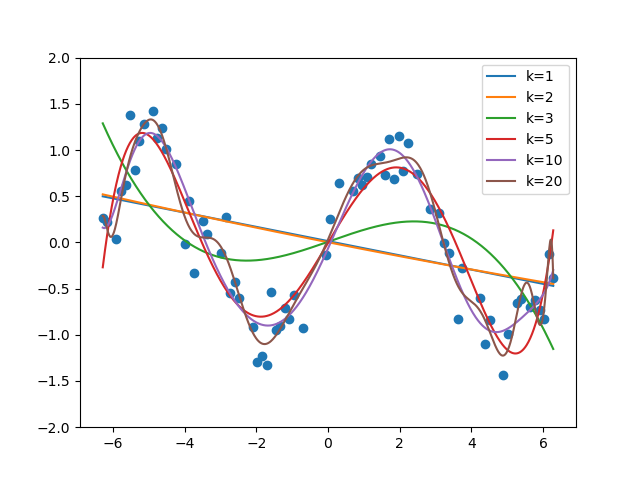
\includegraphics[width=0.65\linewidth]{featuremaps/src/large-poly.png}
  \centering
\caption{Polynomial regression with kernel sizes 1,2,3,5,10 and 20}
\end{figure}

Provide your explanation of the fit for each K value here:\\[50pt]